
%............................
\paragraph{Buried sphere (3D)}

To calculate the pull of gravity, we can use the fact that a sphere has the same
gravitational pull as a point mass located at its centre. The distance between 
the measurement point and the center of the sphere is $\sqrt{x^2+d^2}$, so
\[
g_z = \frac{{\cal G} M_{sphere} d }{(x^2 + d^2)^{3/2}}
\]

radius a=50m, $\Delta \rho=2000$, depth d=100m

$g_z$ has its maximum value directly above the sphere at x=0 m.

%............................
\paragraph{Buried cylinder ()} 

\[
g_z=\frac{2 {\cal G} \pi a^2 d \Delta \rho}{x^2+d^2}
\]
the maximum value of g z is located directly above the axis of the cylinder

g zmax for a cylinder is larger than g zmax for a sphere of the same radius.

Cannot distinguish a buried sphere from a cylinder with just a single profile. Need to
collect gravity on a grid and make a map.

%............................
\paragraph{Buried column (2D)}

\[
g_z=2 {\cal G} \Delta \rho b \ln \frac{r_2}{r_1}
\]

\begin{center}
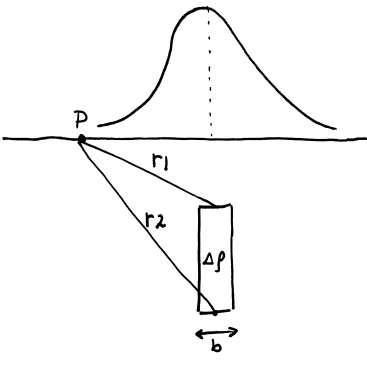
\includegraphics[width=3cm]{images/gravity/column}
\end{center}

%............................
\paragraph{Buried columns (2D)}

\[
g_z=2 {\cal G} \sum_i  \Delta \rho_i  b_i  \ln \frac{r_{2,i}}{r_{1,i}}
\]

\begin{center}
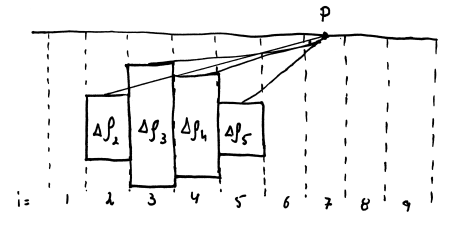
\includegraphics[width=3cm]{images/gravity/columns}
\end{center}





%............................
\paragraph{Uniform layer of rock}

A layer of rock has an infinite extent, thickness $\Delta z$ 
and a density $\rho$. The gravitational
attraction of this slab at the point P at height $z$ obove the layer is 
\[
g_z=2 \pi {\cal G} \rho \Delta z
\]
Note that g z does not depend on the distance from the layer to the measurement point.




